\documentclass[border=3mm,tikz,preview]{standalone}
\usepackage[utf8]{inputenc}
\usepackage{amsmath,amssymb,amsfonts}
\usepackage{graphicx}
\usepackage{tikz}
\usetikzlibrary{shapes.geometric, arrows.meta, positioning, shadows, calc, fit, backgrounds}
\usepackage{xcolor}
\begin{document}

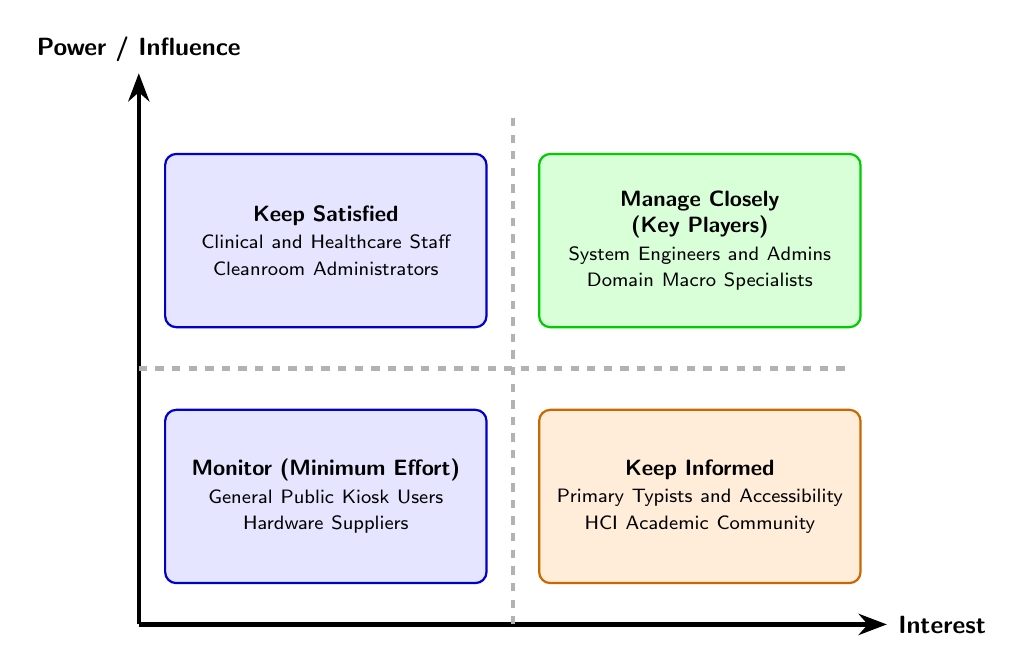
\begin{tikzpicture}[
    box/.style = {rectangle, draw=blue!80!black, fill=blue!10!white, thick, rounded corners=4pt, align=center, font=\sffamily\footnotesize, text width=3.8cm, minimum height=2.2cm, inner sep=4pt},
    gridline/.style = {draw=gray!60, dashed, ultra thick}
]

% Axes
\draw [->, >=Stealth, ultra thick] (0,0) -- (9.5,0) node[right, font=\sffamily\bfseries\small] {Interest};
\draw [->, >=Stealth, ultra thick] (0,0) -- (0,7.0) node[above, font=\sffamily\bfseries\small] {Power / Influence};

% Quadrant Lines
\draw [gridline] (4.75, 0) -- (4.75, 6.5);
\draw [gridline] (0, 3.25) -- (9.0, 3.25);

% Quadrant Labels
\node (q1) [box] at (2.375, 4.875) {\textbf{Keep Satisfied}\\[2pt]\scriptsize Clinical and Healthcare Staff\\\scriptsize Cleanroom Administrators};
\node (q2) [box, fill=green!15!white, draw=green!80!black] at (7.125, 4.875) {\textbf{Manage Closely (Key Players)}\\[2pt]\scriptsize System Engineers and Admins\\\scriptsize Domain Macro Specialists};
\node (q3) [box] at (2.375, 1.625) {\textbf{Monitor (Minimum Effort)}\\[2pt]\scriptsize General Public Kiosk Users\\\scriptsize Hardware Suppliers};
\node (q4) [box, fill=orange!15!white, draw=orange!80!black] at (7.125, 1.625) {\textbf{Keep Informed}\\[2pt]\scriptsize Primary Typists and Accessibility\\\scriptsize HCI Academic Community};

\end{tikzpicture}

\end{document}
